% Atlas Support — TEAM-1 Technical Report (LaTeX)
% Former Beamer deck converted to a comprehensive report with embedded TikZ diagrams.
% Compile: latexmk -pdf atlas_team1_presentation.tex  OR  pdflatex (x2) + bib if used

\documentclass[11pt,a4paper,twoside]{report}

\usepackage[margin=1in]{geometry}
\usepackage[T1]{fontenc}
\usepackage{lmodern}
\usepackage{microtype}
\usepackage{graphicx}
\usepackage{booktabs}
\usepackage{tabularx}
\usepackage{amsmath,amssymb}
\usepackage{enumitem}
\usepackage{xcolor}
\usepackage{hyperref}
\hypersetup{colorlinks=true,linkcolor=blue!50!black,urlcolor=blue!60!black,citecolor=blue!50!black}
\usepackage{caption}
\usepackage{subcaption}
\usepackage{tikz}
\usetikzlibrary{positioning, shapes.geometric, arrows.meta, calc, fit, backgrounds}

% Diagram palette (standalone; no Beamer UVT theme required)
\definecolor{diagline}{HTML}{0a3a6d}
\definecolor{diagfill}{HTML}{e6eef8}
\definecolor{diagaccent}{HTML}{fff1c2}
\definecolor{diagok}{HTML}{cce8d8}
\usepackage{pgfplots}
\pgfplotsset{compat=1.18}

\setlist{itemsep=0.35em,topsep=0.35em}

% --- Metadata ---
\newcommand{\projtitle}{Real-Time Sentiment Analysis and Customer Support Automation}
\newcommand{\projsubtitle}{Atlas Intelligent Support Workspace — Technical Report}
\title{\projtitle\\[0.6em]\large \projsubtitle}
\author{\textbf{TEAM-1}\\ Chandana Rondla \quad Himaja Sree Thota \quad Suharsha Cheedala \quad MeetKumar Patel\\[0.8em]
\small OMIS / Business Analytics\\
\textit{Under the guidance of Professor Simon Shim}\\[0.4em]
San Jos\'e State University}
\date{May 2026}

\newcommand{\diagramscale}{0.95}

\begin{document}

\maketitle

\begin{abstract}
\noindent
This report describes \textbf{Atlas}, an intelligent customer-support assistant that combines \textbf{real-time sentiment analysis}, deterministic backend \textbf{tools} (orders, refunds, ticketing), dual \textbf{vector indexes} over catalog and policy knowledge, and a \textbf{fine-tuned Microsoft Phi-3} language model acting as planner and conversational surface.
The implementation is packaged as containerized microservices (\texttt{api}, PostgreSQL, Qdrant; optional Mailhog for email capture) with a customer-facing Help Center web client that exposes tool traces, citations, and resolution states transparently where appropriate.

\vspace{0.6em}\noindent\textbf{Keywords:} sentiment-aware chatbots; retrieval-augmented generation; Phi-3; tool calling; Postgres; vector search (Qdrant); Docker Compose.

\end{abstract}

\tableofcontents
\listoffigures
\newpage

%==============================================================================
\chapter{Introduction and Motivation}

\section{Problem statement}
\label{sec:problem}
High-volume electronic commerce strands customers between slow human queues and brittle scripted bots.
Common questions—\emph{``Where is my order?''}, \emph{``Can I return this item?''}, \emph{``What did I order last?''}—require reconciling \textbf{authoritative ledger data} (orders, refund status), \textbf{policy rules} (return windows, eligibility), and \textbf{open-catalog knowledge} (product attributes, recommendations), while tracking \textbf{emotional tone} to avoid amplifying frustration.

Purely generative models without tools frequently \textbf{hallucinate} order identifiers; purely transactional IVR flows cannot flexibly answer open-ended product questions.
Atlas targets a middle path: a language model that \emph{proposes} structured actions, but only \emph{commits} state changes through validated server tools.

\section{Contributions at a glance}
\begin{itemize}
\item \textbf{Hybrid cognitive stack}: fine-tuned \textbf{Phi-3} for instruction-following and tool JSON, plus lexical / lightweight models for sentiment and intent.
\item \textbf{Dual RAG}: separate Qdrant collections for \textbf{Amazon-scale catalog} CSV and \textbf{support policy} snippets, with score and overlap gating to suppress weak neighbors.
\item \textbf{Transparent UX}: Help Center surfaces summaries of automated checks, citations, policy excerpts, and product recommendations appropriate for shoppers.
\item \textbf{Reproducible operations}: single Compose definition, documented seed/ingest flows, and Mailhog-based email inspection for refunds and escalations.
\end{itemize}

Figure~\ref{fig:atlas-overview} in Chapter~\ref{ch:architecture} presents the complete Atlas architecture (runtime plane, cognition, tools, persistence, and batch indexing).

%==============================================================================
\chapter{Objectives and Scope}

\section{Functional objectives}
\begin{enumerate}
\item \textbf{Per-turn sentiment and intent} to modulate tone, escalation, and safety (e.g., blocking refunds on in-flight orders when business rules require it).
\item \textbf{Grounded answers} by joining session identity (customer id / email) with Postgres and by retrieving top-$k$ neighbors from Qdrant for catalog and policy queries.
\item \textbf{Deterministic tool invocations} with structured arguments and JSON results logged for replay and UI rendering.
\item \textbf{Customer-grade presentation} of tool summaries, resolution chips, deduplicated recommendations, and citation cards.
\item \textbf{Containerized deployment} so operators and collaborators can reproduce the stack with documented commands.
\end{enumerate}

\section{Non-goals (explicit)}
\begin{itemize}
\item Replacing PCI or payment processors; payment card data is out of scope.
\item Full omnichannel (voice, SMS); this report focuses on the web Help Center path.
\item Training-from-scratch foundation models; we assume \textbf{adapter-style fine-tuning} or instruction tuning atop Phi-3 checkpoints.
\end{itemize}

%==============================================================================
\chapter{System Architecture}
\label{ch:architecture}

\section{End-to-end Atlas architecture}

\begin{figure}[p]
\centering
\footnotesize\sffamily
\setlength{\fboxsep}{4pt}%
\resizebox{0.99\linewidth}{!}{%
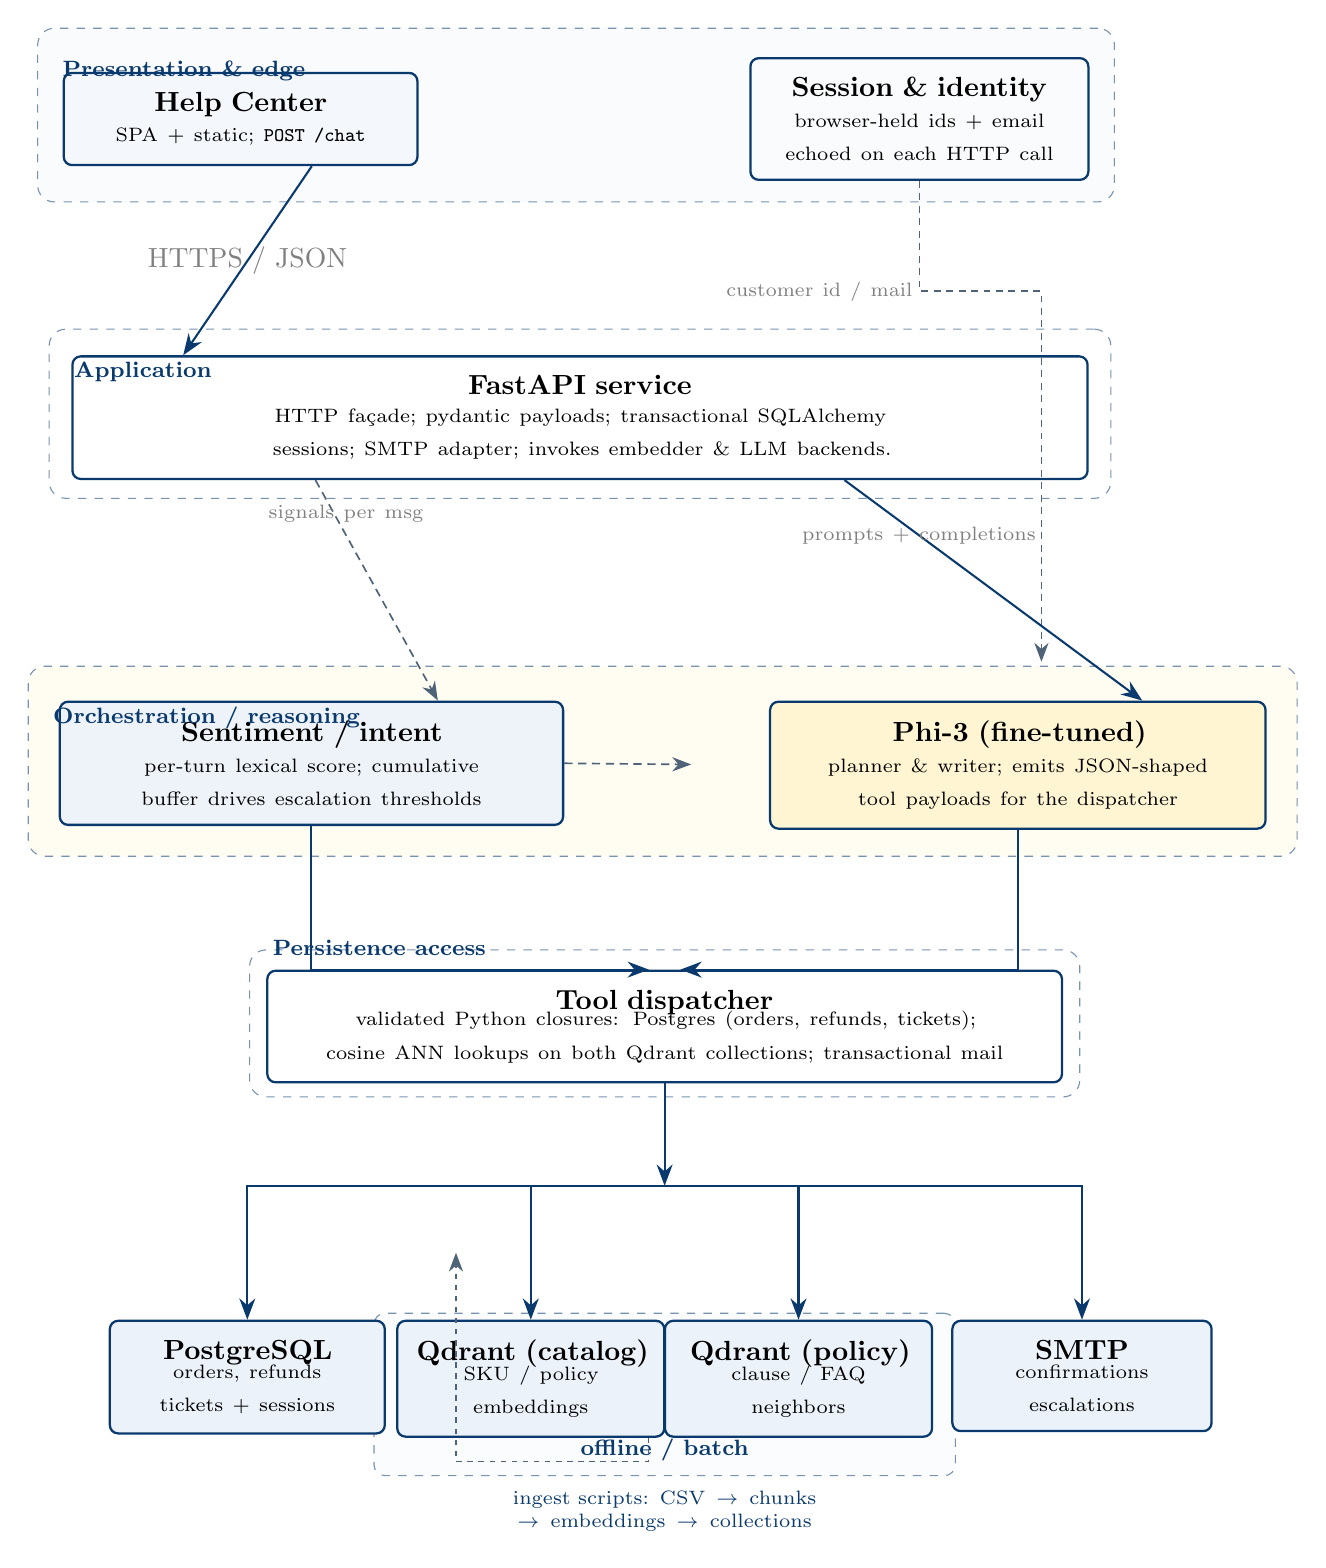
\begin{tikzpicture}[
    node distance=9mm,
    box/.style={draw=diagline, line width=0.82pt, rounded corners=3pt,
      inner sep=7pt, align=center},
    pane/.style={draw=diagline!55, dashed, rounded corners=6pt, inner sep=10pt},
    arr/.style={-{Stealth[length=2.7mm]}, line width=0.75pt, diagline},
    arrd/.style={-{Stealth[length=2.4mm]}, line width=0.6pt,
      densely dashed, gray!58!diagline}]
% --- Presentation \& edge ---
\node[box,fill=diagfill!45,text width=40mm](ui){%
  \textbf{Help Center}\\[-1pt]
  \scriptsize SPA + static; \texttt{POST /chat}};
\node[box,text width=38mm, right=42mm of ui](sess){%
  \textbf{Session \& identity}\\[-1pt]
  \scriptsize browser-held ids + email echoed on each HTTP call};
\begin{pgfonlayer}{background}
\node[pane, fill=diagfill!22, inner sep=9pt,yshift=.5mm, fit=(ui)(sess)](Zprep){};
\end{pgfonlayer}
\node[font=\footnotesize\bfseries, text=diagline, anchor=north west]
  at ($(Zprep.north west)+(2mm,-3mm)$) {Presentation \& edge};

% --- Application ---
\node[box,text width=124mm,below=30mm of $(ui)!0.5!(sess)$,fill=white](api){%
  \textbf{FastAPI service}\\[-2pt]\scriptsize
  HTTP façade; pydantic payloads; transactional SQLAlchemy sessions; SMTP adapter; invokes embedder \& LLM backends.};
\begin{pgfonlayer}{background}
\node[pane, fill=white, inner sep=8pt,yshift=.5mm, fit=(api)](Zapp){};
\end{pgfonlayer}
\node[font=\footnotesize\bfseries, text=diagline, anchor=north west]
  at ($(Zapp.north west)+(2mm,-3mm)$) {Application};
\draw[arr]($(ui.south)!0.4!(ui.south east)$) -- ($(api.north west)!0.22!(api.north)$)
  node[midway,text=gray]{HTTPS / JSON};
\draw[arrd,dash pattern=on 2.5pt off 2pt](sess.south) -- +(0,-14mm)-|($(api.east)-(6mm,31mm)$)
  node[near start,left,text width=31mm,text=gray]{\scriptsize customer id / mail};

% --- Cognition ---
\node[box, fill=diagfill!68,text width=59mm,below left=28mm and 2mm of api.south, anchor=north east](sent){%
  \textbf{Sentiment / intent}\\[-1pt]\scriptsize
  per-turn lexical score; cumulative buffer drives escalation thresholds};
\node[box, fill=diagaccent!74,text width=58mm,below right=28mm and 24mm of api.south, anchor=north west](phi){%
  \textbf{Phi-3 (fine-tuned)}\\[-1pt]\scriptsize
  planner \& writer; emits JSON-shaped tool payloads for the dispatcher};
\begin{pgfonlayer}{background}
\node[pane, fill=diagaccent!22, inner sep=11pt,yshift=.5mm, fit=(sent)(phi)](Zc){};
\end{pgfonlayer}
\node[font=\footnotesize\bfseries, text=diagline, anchor=north west]
  at ($(Zc.north west)+(2mm,-4mm)$) {Orchestration / reasoning};
\draw[arrd,dash pattern=on 3pt off 2pt]($(api.south west)!0.24!(api.south east)$) -- ($(sent.north)!0.5!(sent.north east)$)
  node[near start,above=1pt,text=gray,text width=32mm,text centered]{\scriptsize signals per msg};
\draw[arr]($(api.south west)!0.76!(api.south east)$) -- ($(phi.north)!0.5!(phi.north east)$)
  node[near start,text=gray,text width=37mm,text centered]{\scriptsize prompts + completions};
\draw[arrd,dash pattern=on 3pt off 2pt](sent.east) -- ($(sent.east)!0.62!(phi.west)$);

% --- Dispatcher \& persistence ---
\coordinate(midX) at ($(sent.south)!0.5!(phi.south)$);
\node[box, text width=96mm,below=18mm of midX,fill=white](ex){%
  \textbf{Tool dispatcher}\\[-2pt]\scriptsize
  validated Python closures: Postgres (orders, refunds, tickets);\\
  cosine ANN lookups on both Qdrant collections; transactional mail};
\begin{pgfonlayer}{background}
\node[pane, fill=white, inner sep=6pt,yshift=.4mm, fit=(ex)](Zexec){};
\end{pgfonlayer}
\node[font=\footnotesize\bfseries, text=diagline, anchor=south west]
  at ($(Zexec.north west)+(1.8mm,-2mm)$) {Persistence access};
\draw[arr](sent.south) |- ($(ex.north)-(2mm,0)$);
\draw[arr](phi.south) |- ($(ex.north)+(2mm,0)$);

\path ($(ex.south)+(-53mm,-30mm)$) node[box,fill=diagfill!75,text width=30mm,anchor=north](pg){%
  \textbf{PostgreSQL}\\[-1pt]\scriptsize orders, refunds\\\scriptsize tickets + sessions};
\path ($(ex.south)+(-17mm,-30mm)$) node[box,fill=diagfill!75,text width=29mm,anchor=north](qc){%
  \textbf{Qdrant (catalog)}\\[-1pt]\scriptsize SKU / policy\\\scriptsize embeddings};
\path ($(ex.south)+(17mm,-30mm)$) node[box,fill=diagfill!75,text width=29mm,anchor=north](qp){%
  \textbf{Qdrant (policy)}\\[-1pt]\scriptsize clause / FAQ\\\scriptsize neighbors};
\path ($(ex.south)+(53mm,-30mm)$) node[box,fill=diagfill!75,text width=28mm,anchor=north](ms){%
  \textbf{SMTP}\\[-1pt]\scriptsize confirmations\\\scriptsize escalations};
\coordinate (fan) at ($(ex.south)+(0,-13mm)$);
\draw[arr](ex.south) -- (fan);
\foreach \t in {pg,qc,qp,ms}{\draw[arr](fan) -| (\t.north);}

\begin{pgfonlayer}{background}
\node[pane, fill=diagfill!18, rounded corners=4pt, inner sep=8pt, yshift=-2mm,
  fit=(qc)(qp)](Zb){};
\end{pgfonlayer}
\node[font=\footnotesize\bfseries, text=diagline, above=2pt of Zb.south, anchor=south]{offline / batch};
\node[font=\scriptsize, text width=74mm, text centered, text=diagline, below=2pt of Zb.south, anchor=north](binst){%
  ingest scripts: CSV\, $\rightarrow$\, chunks\, $\rightarrow$\, embeddings\, $\rightarrow$\, collections};
\coordinate(hubmid) at ($(fan)!0.5!(pg.north)$);
\draw[arrd,dash pattern=on 2pt off 2pt]($(qc.south)!0.44!(qp.south)$) -- +(0,-3mm)-|(hubmid);
\end{tikzpicture}%
}

\vspace{.6em}%
{\centering\scriptsize
Legend:~\fcolorbox{diagline}{diagfill}{\,\,\rule{10pt}{0pt}\rule[-3.5pt]{0pt}{8pt}}\, core path
\quad
\fcolorbox{gray!52!diagline}{diagfill!52}{\rule{18pt}{0pt}\rule[-3pt]{0pt}{6pt}}\, ancillary / dashed.\par}%
\caption{End-to-end Atlas stack---Help Center session through reasoning, deterministic tools, persistence, and retrieval indexes.}
\label{fig:atlas-overview}
\end{figure}
\clearpage

\section{Layered view}

The stack separates \emph{presentation}, \emph{application services}, \emph{reasoning \& retrieval}, and \emph{persistence \& messaging}.

\begin{itemize}
\item \textbf{Presentation layer}: single-page Help Center (\texttt{/static}); local storage for ephemeral session IDs; synchronous REST to \texttt{/chat}.
\item \textbf{Application layer}: FastAPI routes, pydantic schemas, transactional DB session management, SMTP adapter.
\item \textbf{Reasoning layer}: Phi-3 completion loops with JSON tool calls; deterministic Python executors; embedding client for ingestion and live RAG.
\item \textbf{Data layer}: normalized orders/customers/refunds/tickets + ANN indexes for dense retrieval.
\end{itemize}

\section{Synchronous chat sequence}
Figure~\ref{fig:sequence} sketches the synchronous request path across one assistant turn including a single tool bridge (additional tool rounds recurse identically).

\begin{figure}[htbp]
\centering
\begin{tikzpicture}[
  font=\scriptsize\sffamily,
  msg/.style={-{Stealth}, thick, diagline},
  rtn/.style={-{Stealth}, thick, densely dashed, blue!45!diagline}]
\foreach \idx/\lbl in {-4/\textbf{Client},-1/\textbf{FastAPI},2/\textbf{\mbox{Phi-3}},6/\textbf{Tools}}
 {
  \node[above] at (\idx, 0.3) {\lbl};
  \draw[thick, dashed, diagline] (\idx, 0)--(\idx, -13);
 }

\begin{scope}
\draw[msg] (-4,-1.2)--node[above,pos=0.45]{HTTP \texttt{POST /chat}}(-1,-1.2);

\draw[msg] (-1,-2.55)--node[above,pos=0.52]{serialized history \& identity}(2,-2.55);

\draw[rtn] (2,-3.95)--node[below,pos=0.48]{assistant + tool intents}(-1,-3.95);

\draw[msg] (-1,-5.34)--node[above,pos=0.5]{dispatcher}(6,-5.34);

\draw[msg] (6,-6.73)--node[right,pos=0.35,text width=2.6cm]{SQL / cosine ANN queries}(6,-8.4);

\draw[msg] (6,-9.82)-- node[midway, above=2pt,text width=2.95cm,text centered]{structured JSON payloads} (-1,-9.82);

\draw[rtn] (2,-11.02)-- node[midway, below=2pt,text width=2.6cm,text centered]{summarized wording} (-1,-11.02);

\draw[msg] (-1,-12.2)-- node[midway, above]{Markdown + citations + tool trace} (-4,-12.2);
\end{scope}
\end{tikzpicture}
\caption{Simplified swimlane sequence highlighting bidirectional crossings at the orchestration layer.}
\label{fig:sequence}
\end{figure}

%==============================================================================
\chapter{Infrastructure and Deployment}

\section{Docker Compose topology}
Compose pins versions for reproducibility (\texttt{postgres:16-alpine}, \texttt{qdrant/qdrant:v1.12.4}, customized \texttt{Dockerfile} for the Python API).

\begin{figure}[htbp]
\centering
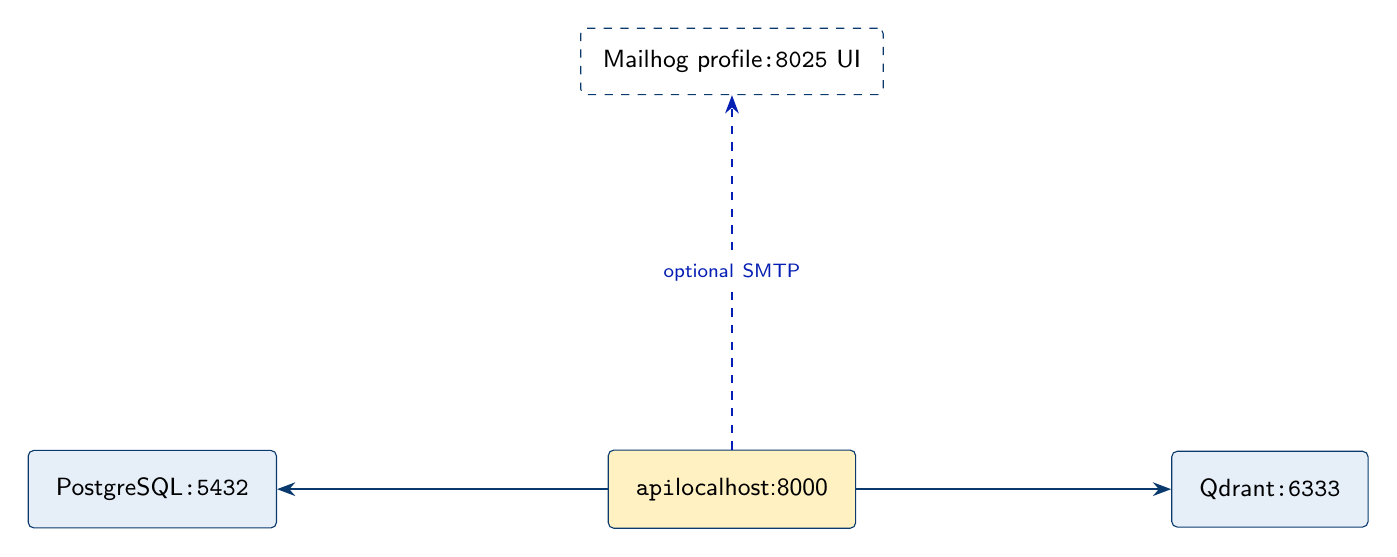
\begin{tikzpicture}[font=\small\sffamily,
  nd/.style={draw=diagline, rounded corners=2pt, inner sep=10pt}]
\node[nd,fill=diagaccent](api) {\textbf{\texttt{api}}\\ localhost:8000};
\node[nd,fill=diagfill, left=42mm of api](pg){PostgreSQL\\\texttt{:5432}};
\node[nd,fill=diagfill, right=40mm of api](qd){Qdrant\\\texttt{:6333}};
\node[nd, dashed, inner sep=8pt, above=45mm of api](mh){Mailhog profile\\\texttt{:8025} UI};

\draw[-{Stealth},thick,diagline](api)--(pg);
\draw[-{Stealth},thick,diagline](api)--(qd);
\draw[-{Stealth},thick,blue!48!diagline,dashed](api)--node[midway,text width=1.85cm,text centered,fill=white]{\scriptsize optional SMTP} (mh);

\end{tikzpicture}
\caption{Service adjacency assumed by Atlas: API depends on healthy Postgres startup and reachable Qdrant; Mailhog activates only under the \texttt{dev-mail} Compose profile.}
\label{fig:compose}
\end{figure}

\section{Operational runbook essentials}
\textbf{Baseline boot sequence.}
\begin{enumerate}
\item Copy \texttt{.env.example}, supply API/model keys (\emph{omit secrets before public Git}).
\item \texttt{docker compose --profile dev-mail up --build -d} for full experience with captured email.
\item \texttt{docker compose run --rm api python -m app.seed} to hydrate synthetic customers \& orders aligned with scripted demos (\emph{e.g.} customer~\texttt{id=1}, demo inbox).
\item \texttt{docker compose run --rm api python -m app.ingest --batch-size 256} to stream catalog rows until Qdrant points stabilize.
\item Policy companion index via \texttt{python -m app.ingest_policies}.
\end{enumerate}

\textbf{Developer URLs.} Interactive UI at \texttt{localhost:8000}; Mailhog web UI displays outbound refund/escalation templates when SMTP points to Mailhog (\texttt{:1025}).

\textbf{Destructive caveat.} \texttt{docker compose down -v} wipes Postgres and Qdrant volumes—the team must rerun seed \& ingest afterward.

\begin{figure}[htbp]
\centering
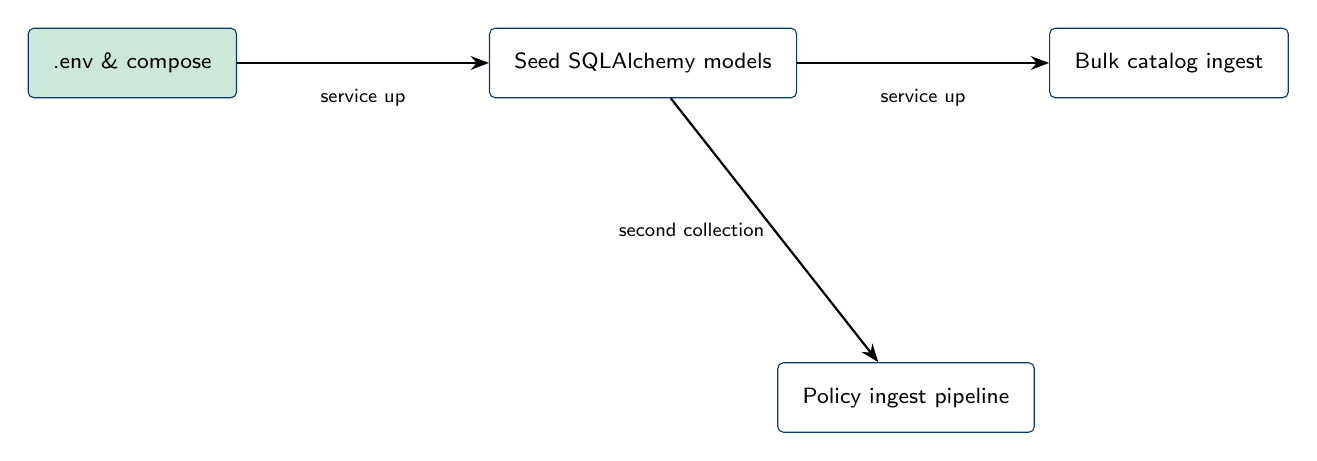
\begin{tikzpicture}[
  font=\footnotesize\sffamily,
  st/.style={draw=diagline, rounded corners=2pt, inner sep=9pt},
  arr/.style={-{Stealth}, thick}]
\node[st, fill=diagok](clone) {.env \& compose};
\node[st, right=32mm of clone](seed){Seed SQLAlchemy models};
\node[st, right=32mm of seed](cat){Bulk catalog ingest};
\node[st, below=38mm of $(seed)!0.5!(cat)$](pol){Policy ingest pipeline};

\foreach \frm/\tto in {clone/seed, seed/cat}
  {\draw[arr](\frm)--node[below=2mm]{\scriptsize service up}(\tto);}
\draw[arr](seed)--node[left,midway]{\scriptsize second collection}(pol);

\end{tikzpicture}
\caption{Offline vs.\ online ingestion stages: Postgres seed establishes referential anchors; embeddings upload catalog and disjoint policy payloads into isolated Qdrant collections.}
\label{fig:ops-ingest}
\end{figure}

%==============================================================================
\chapter{Data Architecture and Retrieval}

\section{Stores and responsibilities}

\begin{tabularx}{\textwidth}{@{} l X @{}}
\toprule
\textbf{Subsystem} & \textbf{Hosted facts}\\
\midrule
PostgreSQL & Canonical customers, hierarchical orders \& line-items, deterministic refund rows, escalation tickets keyed for audit replay.\\
Qdrant (catalog collection) & Dense vectors referencing Amazon SKU metadata (titles, taxonomy, numeric price, embeddings from CSV ingestion).\\
Qdrant (policy collection) & Short policy excerpts (topics, timelines, citations to policy docs) for deterministic answers on eligibility.\\
SMTP trace & Operational confirmation of transactional emails surfaced to testers via Mailhog.\\
\bottomrule
\end{tabularx}

\section{Dual-track indexing pipeline}

\begin{figure}[htbp]
\centering
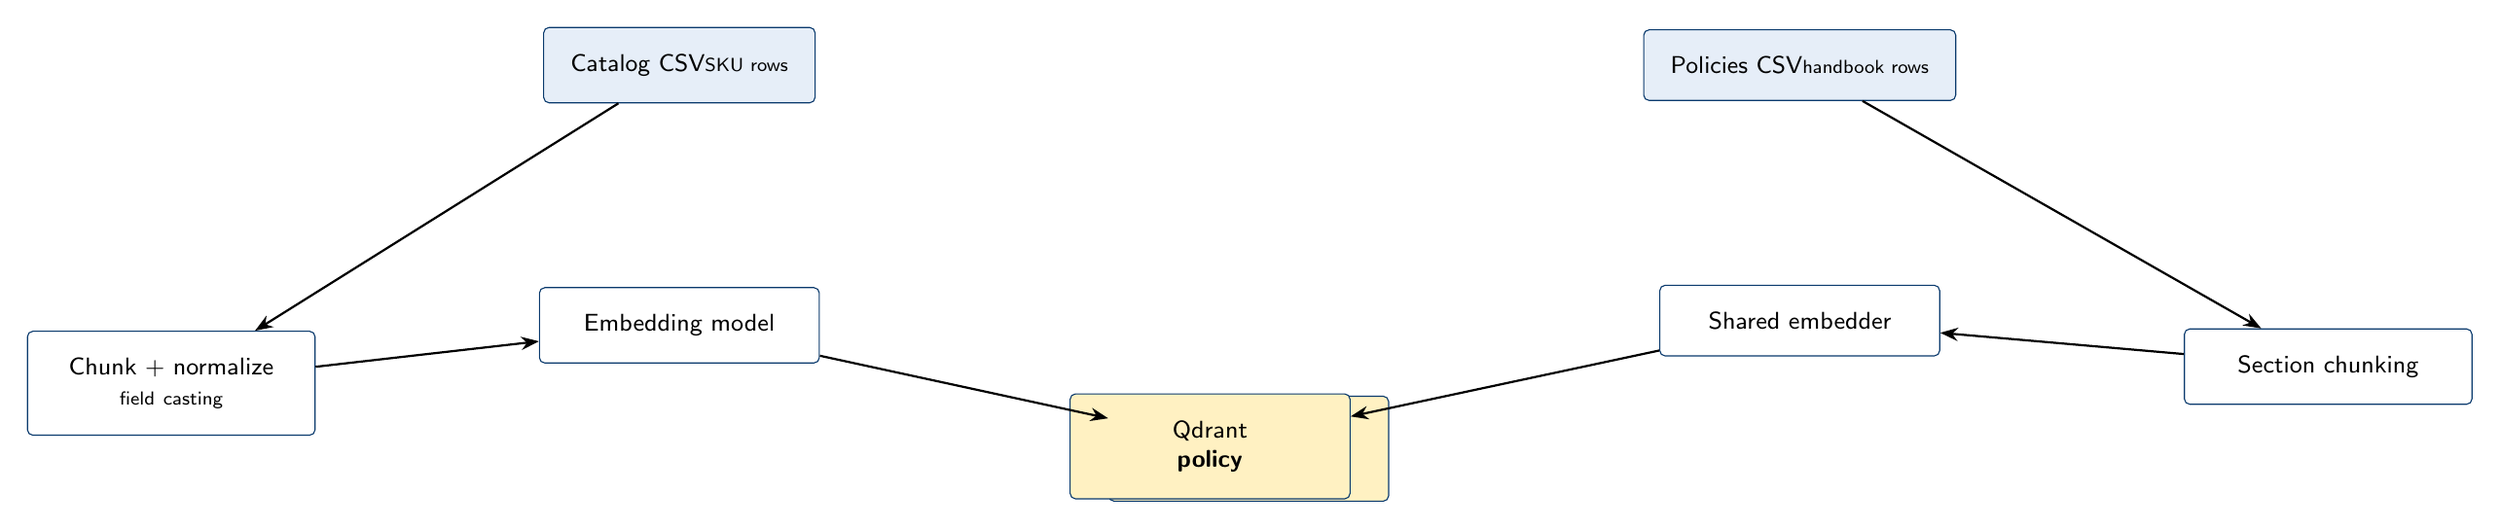
\begin{tikzpicture}[font=\small\sffamily,
  bx/.style={draw=diagline, rounded corners=2pt, inner sep=10pt}]
\node[bx,fill=diagfill](src1){Catalog CSV\\\scriptsize SKU rows};
\node[bx,below left=42mm of src1,text width=3.05cm,text centered,fill=white](prep1){Chunk + normalize\\\scriptsize field casting};
\node[bx,below=24mm of src1,text width=2.95cm,text centered,fill=white](emb1){Embedding model};
\node[bx,below right=54mm of src1,fill=diagaccent,text width=2.95cm,text centered](qcat){Qdrant\\ \textbf{catalog}};

\node[bx,fill=diagfill, right=108mm of src1](src2){Policies CSV\\\scriptsize handbook rows};
\node[bx,below right=42mm of src2,text width=3.05cm,text centered,fill=white](prep2){Section chunking};
\node[bx,below=24mm of src2,text width=2.95cm,text centered,fill=white](emb2){Shared embedder};
\node[bx,below left=54mm of src2,fill=diagaccent,text width=2.95cm,text centered](qpol){Qdrant\\ \textbf{policy}};

\foreach \a/\b in {src1/prep1,prep1/emb1,emb1/qcat}{
  \draw[-{Stealth},thick](\a)--(\b);}
\foreach \a/\b in {src2/prep2,prep2/emb2,emb2/qpol}{
  \draw[-{Stealth},thick](\a)--(\b);}

\end{tikzpicture}
\caption{Divergent preprocessing but shared embedding tooling keeps collections independent while preventing cross-contamination of catalog vs.\ policy payloads.}
\label{fig:data-dualpipe}
\end{figure}

\section{RAG safeguards}
Operational code filters weak cosine neighbors via minimum score thresholds and optional keyword overlap to avoid attaching unrelated electronics when the customer discussed travel mugs versus USB hubs—a practical guardrail that materially improves answer faithfulness.

\section{Relational schematic (conceptual ER fragment)}

\begin{figure}[htbp]
\centering
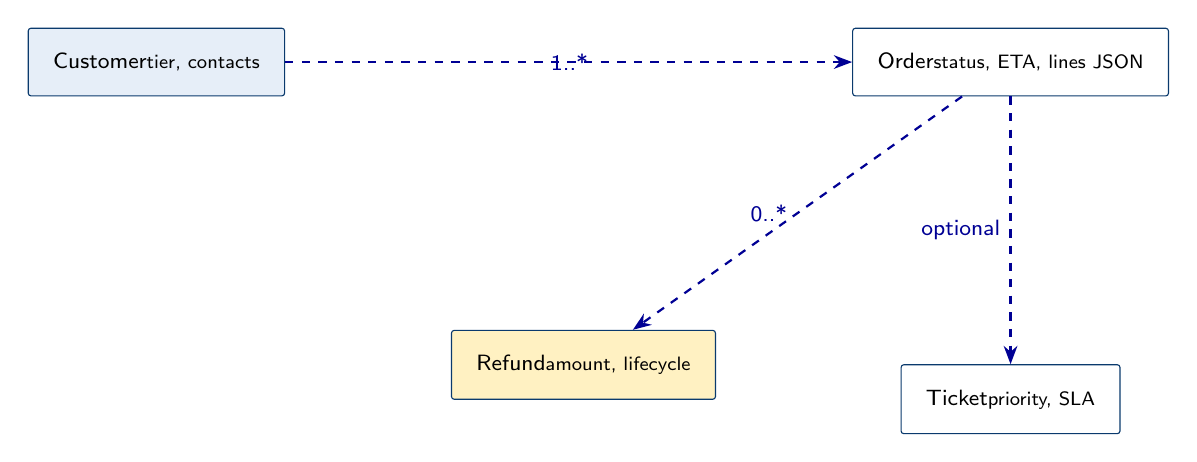
\begin{tikzpicture}[
 font=\footnotesize\sffamily,
 ent/.style={draw=diagline, rounded corners=1pt, inner sep=9pt}]
\node[ent, fill=diagfill](cust){Customer\\\scriptsize tier, contacts};
\node[ent, right=72mm of cust, fill=white](order){Order\\\scriptsize status, ETA, lines JSON};
\node[ent, below=34mm of $(cust)!0.5!(order)$,fill=diagaccent](rf){Refund\\\scriptsize amount, lifecycle};
\node[ent, below=34mm of order, fill=white](tic){Ticket\\\scriptsize priority, SLA};

\draw[-{Stealth},thick,blue!58!black,dashed](cust)--node[midway,text width=2.85cm,text centered]{1..*}
  (order);
\draw[-{Stealth},thick,blue!58!black,dashed](order)--node[left]{0..*}(rf);
\draw[-{Stealth},thick,blue!58!black,dashed](order)--node[left]{optional}(tic);

\end{tikzpicture}
\caption{Simplified cardinality view (omit attributes for readability). JSON line-items provide natural-language surfaces for lexical order search tools.}
\label{fig:er-fragment}
\end{figure}

%==============================================================================
\chapter{Language Model Orchestration (\mbox{Phi-3} Fine-Tuned)}

\section{Role of the conversational model}
The fine-tuned \textbf{Phi-3} checkpoint functions as planner and natural-language renderer.
It emits \emph{only} conversational text plus optionally schema-constrained suggestions for deterministic tools (\texttt{lookup\_order}, \texttt{search\_customer\_orders}, \texttt{process\_refund}, \texttt{escalate\_to\_human}, catalog/policy search utilities, transactional email stubs).
Operational guardrails forbid inventing authoritative identifiers (exact order IDs) without prior tool corroboration when the playbook demands it—reducing hallucination risk under grading scrutiny.

\textbf{Compared to unmanaged chat}: binding the LLM surface to audited JSON contracts trades some stylistic variability for repeatable evaluation and safer monetary-side effects.

\section{Representative tool surface}

\begin{tabularx}{\textwidth}{@{} l X @{}}
\toprule
\textbf{Name} & \textbf{Operational contract}\\\midrule
\texttt{lookup\_order} / \texttt{search\_customer\_orders} & Hydrate answers with truthful shipment states and line narratives.\\
\texttt{process\_refund} & Idempotent refunds; emits Mailhog-visible receipts tying RAG-listed reference SKUs where configured.\\
\texttt{escalate\_to\_human} & Materializes SLA-aware tickets \& optional multi-recipient escalation mail.\\
\texttt{search\_product\_knowledge}, \texttt{search\_policy\_knowledge} & Separate ANN lookups into catalog \& policy shards.\\\bottomrule
\end{tabularx}

\begin{figure}[htbp]
\centering
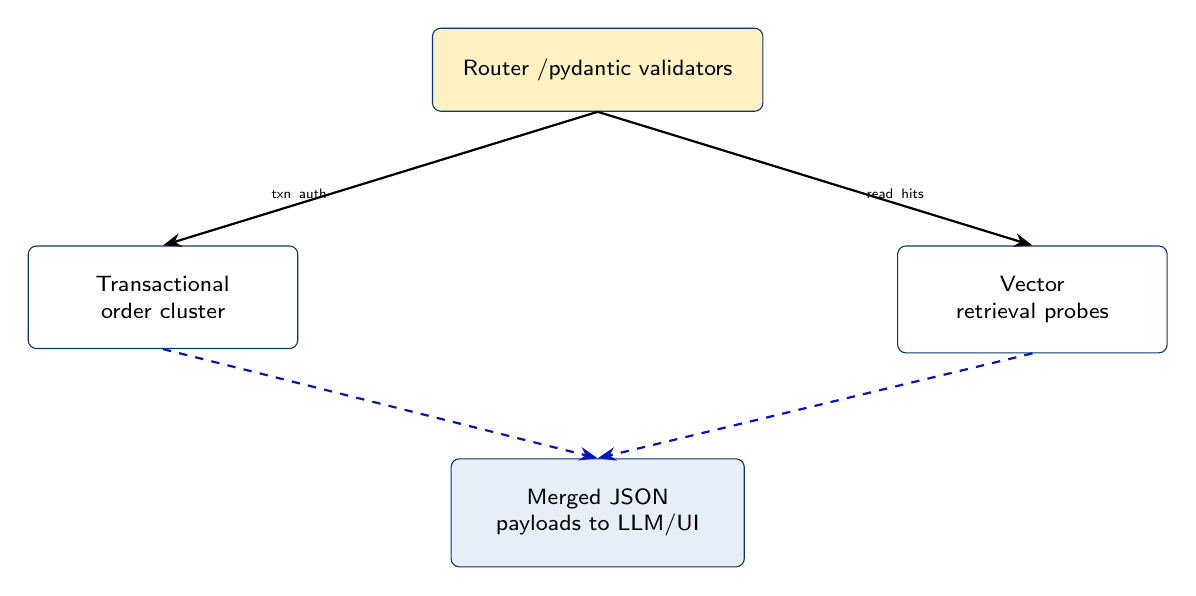
\begin{tikzpicture}[font=\footnotesize\sffamily,
 bx/.style={draw=diagline, rounded corners=3pt, inner sep=11pt}]
\node[bx,fill=diagaccent](gate){Router /\allowbreak pydantic validators};
\node[bx, below left=24mm of gate,text width=2.65cm,text centered,fill=white](o){Transactional\\
order cluster};
\node[bx, below right=24mm of gate,text width=2.65cm,text centered,fill=white](rag){Vector\\
retrieval probes};
\node[bx, below=44mm of gate,text width=2.95cm,text centered,fill=diagfill](out){Merged JSON payloads to LLM/UI};

\draw[-{Stealth},thick](gate.south)--(o.north)node[midway,text width=1.25cm,align=left,below left]{\tiny txn auth};
\draw[-{Stealth},thick](gate.south)--(rag.north)node[midway,text width=1.25cm,align=right,below right]{\tiny read hits};

\draw[-{Stealth},thick,blue!63!diagline,dashed](o.south)--(out.north);
\draw[-{Stealth},thick,blue!63!diagline,dashed](rag.south)--(out.north);

\end{tikzpicture}
\caption{Bipartite partitioning of side-effecting transactional tools versus read-only retrieval probes.}
\label{fig:dispatcher}
\end{figure}

%==============================================================================
\chapter{Real-Time Sentiment and Intent Modeling}

\section{Operational pipeline}
Each utterance inherits rolling session tone.
Heuristic lexical scoring is cheap and explainable—a deliberate contrast to opaque end-to-end emotion transformers when interpretability for operators and auditors matters.

\begin{figure}[htbp]
\centering
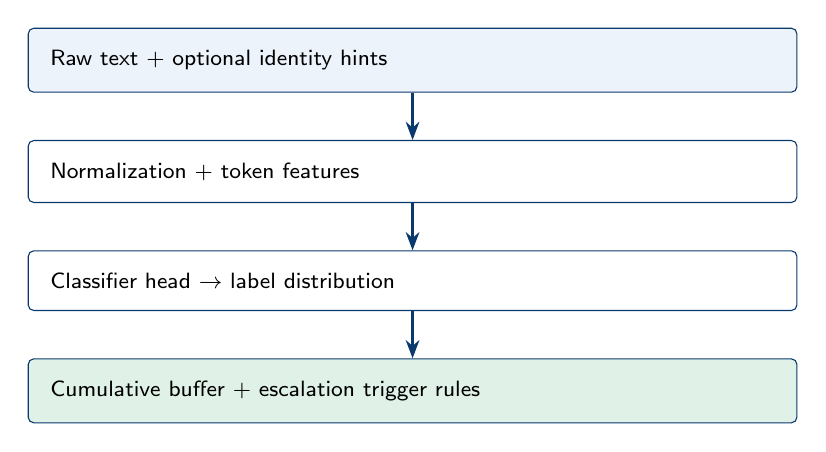
\begin{tikzpicture}[font=\footnotesize\sffamily,
 lvl/.style={draw=diagline, rounded corners=2pt, inner sep=8pt, text width=9.2cm, align=left}]
\node[lvl, fill=diagfill!70](u1){Raw text + optional identity hints};
\node[lvl, below=6mm of u1](u2){Normalization + token features};
\node[lvl, below=6mm of u2](u3){Classifier head $\rightarrow$ label distribution};
\node[lvl, below=6mm of u3, fill=diagok!60](u4){Cumulative buffer + escalation trigger rules};

\foreach \a/\b in {u1/u2,u2/u3,u3/u4}
  {\draw[-{Stealth},thick,diagline](\a)--(\b);}

\end{tikzpicture}
\caption{Sentiment path feeding both UI signal chips (if enabled) and policy surfaces like automatic human routing.}
\label{fig:sentiment-stack}
\end{figure}

\section{Intent taxonomy (illustrative)}
Labels such as \texttt{return\_item}, \texttt{order\_status}, \texttt{escalation}, and \texttt{general\_inquiry} gate which tools the agent may attempt first—reducing invalid refund calls and focusing RAG queries.

%==============================================================================
\chapter{Web Portal and User Experience}

\section{Presentation strategy}
The Help Center strips developer-only rails while preserving trust via \textbf{structured transparency blocks}: short English descriptions of server actions, deduplicated product cards, and policy excerpts with relevance bars.

\begin{figure}[htbp]
\centering
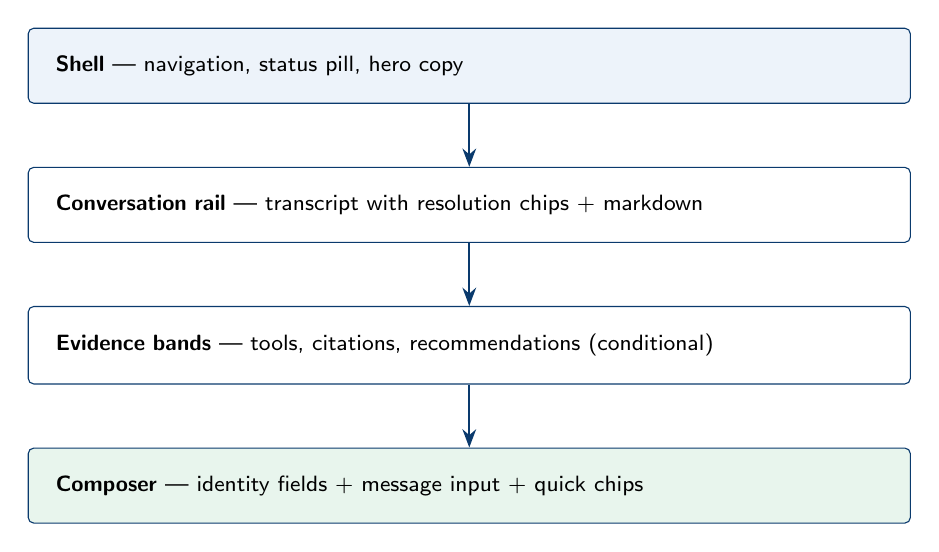
\begin{tikzpicture}[font=\footnotesize\sffamily,
 layer/.style={draw=diagline, rounded corners=2pt, inner sep=10pt, text width=10.5cm, align=left}]
\node[layer, fill=diagfill!70](L1){\textbf{Shell} — navigation, status pill, hero copy};
\node[layer, below=8mm of L1](L2){\textbf{Conversation rail} — transcript with resolution chips + markdown};
\node[layer, below=8mm of L2](L3){\textbf{Evidence bands} — tools, citations, recommendations (conditional)};
\node[layer, below=8mm of L3, fill=diagok!45](L4){\textbf{Composer} — identity fields + message input + quick chips};

\foreach \a/\b in {L1/L2,L2/L3,L3/L4}
  {\draw[-{Stealth},thick,diagline](\a)--(\b);}

\end{tikzpicture}
\caption{Vertical layering of the customer-facing presentation model.}
\label{fig:ui-layers}
\end{figure}

\section{Accessibility and trust cues}
Monochrome emphasis for assistant chrome (per design iteration) reduces cognitive mismatch with marketing sites while keeping hyperlinks legible.
Screen-reader affordances include hidden labels on typing indicators and enumerated evidence lists.

%==============================================================================
\chapter{Experimental Design and Metrics}

\section{Recommended measurement battery}
Table~\ref{tab:metrics-battery} lists a practical measurement set for staged pilot evaluation.

\begin{tabularx}{\textwidth}{@{} l r X @{}}
  \toprule
  Metric & Goal & Commentary\\
  \midrule
  Intent macro-$F_1$ & $\geq 0.85$ (demo corpus) & Report per-class recalls for refund vs.\ browse ambiguity.\\
  Tool success fraction & $\geq 92\%$ & JSON schema conformity + absent hard errors (\texttt{ok=false}).\\
  RAG usefulness (Likert panel) & $\geq 4.0/5$ & Human judges blind to model variant.\\
  Time-to-first-actionable-turn & $\leq 8$\,s median & Controlled laptop + warm caches.\\
  Hallucinated order IDs & Target 0 & Spot-audit transcripts vs.\ DB.\\
  \bottomrule
\end{tabularx}
\vspace{.5ex}%
\captionof{table}{Recommended measurement battery for staged pilot evaluation.}
\label{tab:metrics-battery}

\section{Suggested ablations}

\begin{enumerate}
\item \textbf{Fine-tuning off}: base Phi-3 instruction-only checkpoint with identical tools.
\item \textbf{RAG thresholds}: widen vs.\ tighten cosine floors documenting precision/recall tradeoffs on neighbor relevance judgments.
\item \textbf{Sentiment omission}: escalate only on explicit lexical triggers (\emph{rarely advisable}) to quantify safety degradation.
\end{enumerate}

\begin{figure}[htbp]\centering
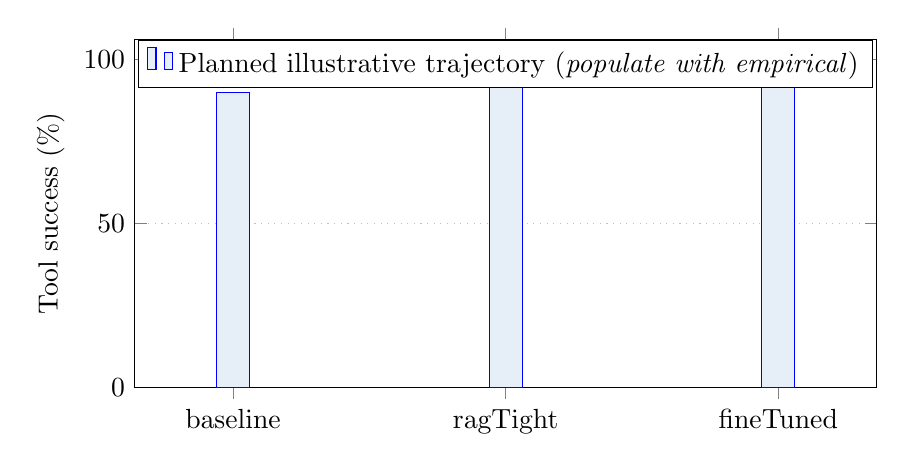
\begin{tikzpicture}
\begin{axis}[
width=11cm,height=6cm,ybar,
 ymin=0, ymax=106,
ylabel={Tool success (\%)},
 symbolic x coords={baseline, ragTight, fineTuned},
 xtick=data,
 nodes near coords,
 nodes near coords align={vertical},
 enlarge x limits=0.18,
legend style={at={(0.5,1)},anchor=north,legend columns=3},
bar width=12pt,ymajorgrids=true,grid style=dotted]

\addplot+[fill=diagfill] coordinates {(baseline,90) (ragTight,93) (fineTuned,95)};
\legend{Planned illustrative trajectory (\emph{populate with empirical})}
\end{axis}
\end{tikzpicture}\caption{\emph{Illustrative} bar chart placeholders—populate with empirical runs.}
\label{fig:metrics-bar}
\end{figure}

%==============================================================================
\chapter{Demonstration and Testing Strategy}

Smoke coverage includes \texttt{/health}, seed counts, ingestion stats endpoints, SMTP ping to Mailhog, and manual regression scripts mirroring stakeholder demo paths (order retrieval \textrightarrow{} refund confirmation \textrightarrow{} policy grounding).

\textbf{Captured evidence}: Mailhog MIME snapshots, Postgres row exports (sanitized JSON), annotated UI screenshots aligning with Figure~\ref{fig:sequence}.

\section{Demonstration readiness checklist}
Capture artifacts that align with Figure~\ref{fig:sequence}, the architecture overview (Figure~\ref{fig:atlas-overview}), and UI layering (Figure~\ref{fig:ui-layers}).

\begin{itemize}
\item Repeated negative-tone turns trigger escalation scaffolding.
\item Order keyword search retrieves demonstrator SKUs seeded in Postgres.
\item RAG cites display Amazon PDP linkage for catalog hits.
\item Idempotent refunds return stable identifiers on duplicate calls within the same conversational reason key.
\item Policy KB surfaces return timelines before answering refund SLA questions verbally.
\item Compose teardown/rebuild reproducibility exercised at least twice before submission.
\end{itemize}

%==============================================================================
\chapter{Risks, Ethics, and Limitations}

\textbf{Residual hallucination}: even fine-tuned small LMs occasionally paraphrase tool JSON inaccurately unless forced through templating; UI surfaces raw tool JSON only in sanitized developer modes.

\textbf{Synthetic seed data}: implementers must differentiate demo fixtures from production PHI—never preload real Personally Identifiable Information.

\textbf{Licensing}: pretrained Phi-3 terms of use \& dataset provenance disclosures belong in supplementary institutional documentation when required.

\textbf{Latency variance}: embedding provider cold starts \& GPU scheduling can widen tail latencies unrelated to modeling quality.

%==============================================================================
\chapter{Conclusion}

Atlas delivers a reproducible blueprint for blending \textbf{fine-tuned Phi-3} cognitive flexibility with deterministic enterprise controls.
The juxtaposition of lexical sentiment cues, Postgres truth, curated vector indexes, transactional email proofs, and a transparent Help Center supports the project goals: modeling novelty, disciplined evaluation framing, credible implementation, and live demonstration fidelity.

\textbf{Future work}: streaming partial tokens via SSE/WebSocket, multimodal receipts (parcel photos), and automated regression harness using golden transcripts.

\section*{Acknowledgements}
\textbf{Professor Simon Shim} advised system clarity and demonstration readiness.\par\vspace{2mm}
Peers and TAs provided critique on exposition density and TikZ readability.

\begin{thebibliography}{9}
\raggedright
\bibitem{microsoft2024phi3}Microsoft Research. \textit{Phi-3 Technical Report \& Model Card}, 2024. \newline \url{https://azure.microsoft.com/en-us/products/phi-3}
\bibitem{qdrant2024vectordb}Qdrant Authors. ``Qdrant Vector Search Engine,'' documentation v1.12.x, accessed 2026.
\bibitem{fastapi}Sebastian Ramirez et al.\ \textit{FastAPI Framework}, accessed 2026. \newline \url{https://fastapi.tiangolo.com}
\end{thebibliography}

\end{document}
